\documentclass[aspectratio=169,10pt]{beamer}
\usetheme{gotham}
\usepackage{helvet}
\renewcommand{\familydefault}{\sfdefault}

\usepackage{tikz}
\usetikzlibrary{shapes.geometric,arrows.meta,positioning,calc,fit}
\usepackage{xcolor}
\usepackage{graphicx}\graphicspath{{./}}
\usepackage{booktabs}
\usepackage{amsmath}
\usepackage{array}
\usepackage{hyperref}

% ---------- UTM-inspired palette ----------
\definecolor{UTBlue}{HTML}{1E3765}
\definecolor{Pantone633}{HTML}{007FA3}
\definecolor{Pantone2985}{HTML}{6FC7EA}
\definecolor{PantoneWarmRed}{HTML}{DC4633}
\definecolor{Pantone227}{HTML}{AB1368}
\definecolor{SoftBlue}{HTML}{EAF4F8}
\definecolor{SoftGrey}{HTML}{F4F5F7}
\definecolor{TextGrey}{HTML}{3D4650}
\definecolor{WarmYellow}{HTML}{F8E9A1}

% ---------- Theme tuning ----------
\gothamset{
  numbering=framenumber,
  parttocframe default=off,
  sectiontocframe default=off,
  subsectiontocframe default=off
}
\setbeamercolor{progress bar}{fg=UTBlue,bg=UTBlue!25}
\setbeamercolor{frametitle}{bg=UTBlue,fg=white}
\setbeamercolor{normal text}{fg=TextGrey,bg=white}
\setbeamercolor{alerted text}{fg=PantoneWarmRed}
\setbeamertemplate{navigation symbols}{}
\setbeamerfont{frametitle}{family=\sffamily,series=\bfseries,size=\large}
\setbeamerfont{title}{family=\sffamily,series=\bfseries}
\setbeamerfont{subtitle}{family=\sffamily,series=\bfseries}

% ---------- Custom TOC circles ----------
\defbeamertemplate{section in toc}{teal circles}{%
  \leavevmode%
  \begin{beamercolorbox}[sep=-0.5pt,left]{section in toc}%
    \tikz[baseline=(tocprefix.base)]{
      \node[circle,fill=Pantone633,inner sep=2.2pt,text=white]
      (tocprefix) {\small\inserttocsectionnumber};
    }%
    \hspace{0.65em}\inserttocsection\par%
  \end{beamercolorbox}%
}
\setbeamertemplate{section in toc}[teal circles]
\setcounter{tocdepth}{1}
\AtBeginSection[]{}

% ---------- Frame title and footline ----------
% Standard slides: UTM/MCS wordmark sits in the top-left of the title bar.
\setbeamertemplate{frametitle}{%
  \nointerlineskip%
  \begin{beamercolorbox}[wd=\paperwidth,ht=0.86cm,dp=0.18cm,leftskip=0.36cm]{frametitle}%
    \raisebox{-0.05cm}{
\includegraphics[height=0.42cm]{UTM-MCS-logo-white-clean.png}}%
    \hspace{0.55cm}%
    {\sffamily\bfseries\large\insertframetitle}%
  \end{beamercolorbox}%
}

\defbeamertemplate{footline}{slide number only}{%
  \hfill\insertframenumber\hspace*{0.6em}\vskip0.35em%
}
\setbeamertemplate{footline}[slide number only]

% ---------- Helpers ----------
\newcommand{\key}[1]{\textcolor{Pantone633}{\textbf{#1}}}
\newcommand{\muted}[1]{\textcolor{TextGrey!72}{#1}}

\newcommand{\screenshotplaceholder}[2][0.78\textwidth]{%
  \begin{center}
  \begin{tikzpicture}
    \node[
      draw=Pantone633!55,
      line width=0.8pt,
      rounded corners=3pt,
      fill=SoftGrey,
      text width=0.70\textwidth,
      minimum height=3.9cm,
      align=center,
      inner sep=10pt
    ] {\textcolor{Pantone633}{\Large\textbf{Screenshot placeholder}}\\[0.5em]
       \normalsize #2};
  \end{tikzpicture}
  \end{center}
}

\newcommand{\smallplaceholder}[1]{%
  \begin{tikzpicture}
    \node[
      draw=Pantone633!45,
      rounded corners=3pt,
      fill=SoftGrey,
      minimum width=0.27\textwidth,
      minimum height=2.55cm,
      align=center,
      inner sep=6pt
    ] {\small\textcolor{Pantone633}{\textbf{#1}}};
  \end{tikzpicture}%
}

\newcommand{\card}[3]{%
  \begin{tikzpicture}
    \node[
      draw=#1!55,
      fill=#1!7,
      rounded corners=4pt,
      inner sep=10pt,
      text width=0.255\textwidth,
      minimum height=1.78cm,
      align=left
    ] {\textcolor{#1}{\textbf{#2}}\\[0.35em]\scriptsize #3};
  \end{tikzpicture}%
}

% ---------- Title metadata ----------
\title{Developing Interactive Instructional Resources for STA258 Using Quarto}
\subtitle{Statistics with Applied Probability}
\author{Ashwin Selvapandian, Sarah Halime}
\date{Department of Mathematical and Computational Sciences\\University of Toronto Mississauga}

\begin{document}

% ============================================================
% Slide 1 -- Title
% ============================================================
\begin{frame}[plain]
\vspace*{1.0em}
\begin{tikzpicture}[remember picture,overlay]
  \fill[SoftGrey] (current page.south west) rectangle (current page.north east);
  \fill[UTBlue] (current page.north west) rectangle ([yshift=-0.16cm]current page.north east);
  \fill[UTBlue] (current page.south west) rectangle ([yshift=0.12cm]current page.south east);
\end{tikzpicture}

\begin{tikzpicture}[remember picture,overlay]
  \node[anchor=north west] at ([xshift=0.55cm,yshift=-0.45cm]current page.north west)
    {
\includegraphics[width=0.22\paperwidth]{UTM-MCS-logo-transparent.png}};
  \node[anchor=south east] at ([xshift=-0.65cm,yshift=0.55cm]current page.south east)
    {
\includegraphics[width=0.14\paperwidth]{STA258_cat_logo.png}};
\end{tikzpicture}

\vspace*{2.7em}
\begin{center}
\begin{beamercolorbox}[rounded=false,sep=0.65em,wd=0.93\paperwidth,center]{block body}
{\sffamily\fontsize{17.8}{21.5}\selectfont\color{UTBlue}\textbf{Developing Interactive Instructional Resources\\for STA258 Using Quarto}}
\end{beamercolorbox}

\vspace{0.65em}
{\large\color{Pantone633}\textbf{Statistics with Applied Probability}}

\vspace{0.75em}
{\normalsize Ashwin Selvapandian, Sarah Halime}

\vspace{0.5em}
{\small\muted{Department of Mathematical and Computational Sciences}}\\[-0.05em]
{\small\muted{University of Toronto Mississauga}}
\end{center}
\vspace{0.35em}
\end{frame}

% ============================================================
% Slide 2 -- TOC
% ============================================================
\begin{frame}{Table of contents}
\vspace*{0.8em}
\tableofcontents
\end{frame}

% ============================================================
\section{Motivation and goals}
% ============================================================

% Slide 3
\begin{frame}{Why this project?}
\vspace{0.4em}
\begin{columns}[T,onlytextwidth]
\column{0.52\textwidth}
\normalsize
A statistics course asks students to move repeatedly between:
\vspace{0.6em}
\begin{itemize}
  \item mathematical ideas,
  \item interpretation in context,
  \item visualization,
  \item computation in R, and
  \item practice and feedback.
\end{itemize}

\column{0.44\textwidth}
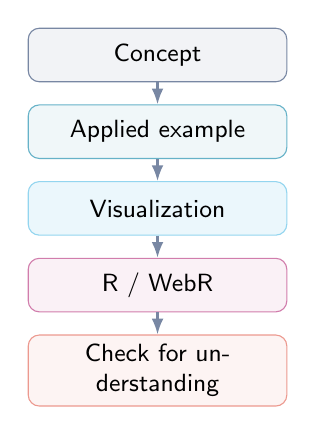
\begin{tikzpicture}[node distance=0.28cm, every node/.style={font=\small}]
  \node[draw=UTBlue!60,fill=UTBlue!6,rounded corners=4pt,text width=3.05cm,align=center,minimum height=0.68cm] (a) {Concept};
  \node[draw=Pantone633!60,fill=Pantone633!6,rounded corners=4pt,text width=3.05cm,align=center,minimum height=0.68cm,below=of a] (b) {Applied example};
  \node[draw=Pantone2985!75,fill=Pantone2985!14,rounded corners=4pt,text width=3.05cm,align=center,minimum height=0.68cm,below=of b] (c) {Visualization};
  \node[draw=Pantone227!55,fill=Pantone227!6,rounded corners=4pt,text width=3.05cm,align=center,minimum height=0.68cm,below=of c] (d) {R / WebR};
  \node[draw=PantoneWarmRed!55,fill=PantoneWarmRed!6,rounded corners=4pt,text width=3.05cm,align=center,minimum height=0.68cm,below=of d] (e) {Check for understanding};
  \draw[-{Latex[length=2mm]},thick,UTBlue!60] (a)--(b);
  \draw[-{Latex[length=2mm]},thick,UTBlue!60] (b)--(c);
  \draw[-{Latex[length=2mm]},thick,UTBlue!60] (c)--(d);
  \draw[-{Latex[length=2mm]},thick,UTBlue!60] (d)--(e);
\end{tikzpicture}
\end{columns}

\vspace{0.15em}
\begin{beamercolorbox}[rounded=true,sep=0.8em,wd=\textwidth]{block body}
\centering\textbf{Project aim:} bring these steps into one coherent, browser-based learning experience.
\end{beamercolorbox}
\end{frame}

% Slide 4
\begin{frame}{Design goals}
\vspace{0.35em}
\begin{columns}[T,onlytextwidth]
\column{0.48\textwidth}
\textcolor{UTBlue}{\textbf{Clarity}}\
Keep statistical reasoning visible with concise explanations and deliberate visual hierarchy.

\vspace{0.6em}
\textcolor{Pantone633}{\textbf{Interactivity}}\
Let students calculate, visualize, run R, and check understanding directly inside the slides.

\vspace{0.6em}
\textcolor{Pantone227}{\textbf{Consistency}}\
Use a common structure, visual language, and interaction pattern across the course.

\column{0.48\textwidth}
\textcolor{PantoneWarmRed}{\textbf{Applied context}}\
Anchor procedures in realistic examples before formal computation.

\vspace{0.6em}
\textcolor{Pantone2985!80!black}{\textbf{Reproducibility}}\
Keep source, computation, styling, and publishing within a maintainable workflow.

\vspace{0.6em}
\textcolor{Pantone633}{\textbf{Accessibility}}\
Reduce software barriers by moving core interactions into the browser.
\end{columns}

\vspace{0.55em}
\begin{beamercolorbox}[rounded=true,sep=0.7em,wd=\textwidth]{block body}
\centering The design goal was not to make slides ``more interactive'' in isolation, but to make the learning sequence more coherent.
\end{beamercolorbox}
\end{frame}

% Slide 5
\begin{frame}{What we built}
\vspace{0.45em}
\begin{columns}[T,onlytextwidth]
\column{0.48\textwidth}
\begin{beamercolorbox}[rounded=true,sep=0.85em,wd=\textwidth]{block body}
\textcolor{UTBlue}{\textbf{Chapter-based course structure}}\\[0.35em]
\small Chapter landing pages and browser-based slide decks organized across the STA258 course sequence.
\end{beamercolorbox}

\vspace{0.7em}
\begin{beamercolorbox}[rounded=true,sep=0.85em,wd=\textwidth]{block body}
\textcolor{Pantone227}{\textbf{Interactive computation}}\\[0.35em]
\small WebR, R demonstrations, solution reveals, and quiz interactions embedded directly within the learning materials.
\end{beamercolorbox}

\column{0.48\textwidth}
\begin{beamercolorbox}[rounded=true,sep=0.85em,wd=\textwidth]{block body}
\textcolor{Pantone633}{\textbf{Statistical visualization}}\\[0.35em]
\small Reproducible R graphics, Plotly figures, and selected JavaScript widgets designed around applied examples.
\end{beamercolorbox}

\vspace{0.7em}
\begin{beamercolorbox}[rounded=true,sep=0.85em,wd=\textwidth]{block body}
\textcolor{PantoneWarmRed}{\textbf{A maintainable publishing system}}\\[0.35em]
\small Shared CSS, Git/GitHub workflow, rendered HTML/PDF access, and documentation for future maintainers.
\end{beamercolorbox}
\end{columns}
\end{frame}

% Slide 6
\begin{frame}{The learning sequence}
\vspace{1.0em}
\begin{center}
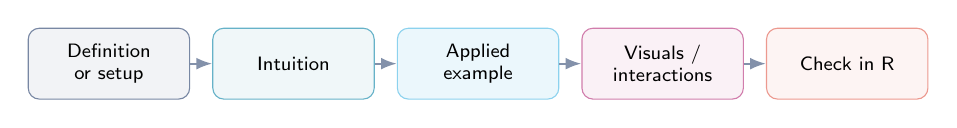
\begin{tikzpicture}[node distance=0.28cm, every node/.style={font=\scriptsize}]
  \node[draw=UTBlue!60,fill=UTBlue!6,rounded corners=4pt,minimum width=2.05cm,minimum height=0.9cm,align=center] (d) {Definition\\or setup};
  \node[draw=Pantone633!60,fill=Pantone633!6,rounded corners=4pt,minimum width=2.05cm,minimum height=0.9cm,align=center,right=of d] (i) {Intuition};
  \node[draw=Pantone2985!80,fill=Pantone2985!14,rounded corners=4pt,minimum width=2.05cm,minimum height=0.9cm,align=center,right=of i] (e) {Applied\\example};
  \node[draw=Pantone227!55,fill=Pantone227!6,rounded corners=4pt,minimum width=2.05cm,minimum height=0.9cm,align=center,right=of e] (p) {Visuals /\\interactions};
  \node[draw=PantoneWarmRed!55,fill=PantoneWarmRed!6,rounded corners=4pt,minimum width=2.05cm,minimum height=0.9cm,align=center,right=of p] (r) {Check in R};
  \foreach \x/\y in {d/i,i/e,e/p,p/r}{\draw[-{Latex[length=2mm]},thick,UTBlue!55] (\x)--(\y);}
\end{tikzpicture}
\end{center}

\vspace{1.0em}
\begin{itemize}
  \item Repeating the same structure gives students a \key{predictable rhythm} from one topic to the next.
  \item Interactive elements appear where students can apply or check their understanding of the statistical idea.
\end{itemize}
\end{frame}

% ============================================================
\section{Building the resource}
% ============================================================



% Slide 7
\begin{frame}{Technical stack}
\vspace{0.35em}
\small
\begin{columns}[T,onlytextwidth]
\column{0.47\textwidth}
\begin{itemize}
  \item \key{Quarto} for authoring and rendering
  \item \key{Reveal.js} for browser-based presentations
  \item \key{R / knitr} for reproducible calculations and figures
  \item \key{WebR} for live R execution in the browser
  \item \key{Plotly} and JavaScript for interactive visualizations
\end{itemize}

\column{0.47\textwidth}
\begin{itemize}
  \item \key{HTML/CSS} for custom layouts and interaction design
  \item \key{Quiz plugins} for embedded formative checks
  \item \key{Git/GitHub} for collaborative version control
  \item \key{GitHub Pages} for deployment
  \item \key{PDF views} for printable / static access
\end{itemize}
\end{columns}

\vspace{0.45em}
\begin{beamercolorbox}[rounded=true,sep=0.65em,wd=\textwidth]{block body}
\centering
The result is one workflow from \textbf{source code} $\rightarrow$ \textbf{computation} $\rightarrow$ \textbf{interaction} $\rightarrow$ \textbf{published course resource}.
\end{beamercolorbox}
\end{frame}

% Slide 8
\begin{frame}{A consistent visual system}
\vspace{0.35em}
\begin{columns}[T,onlytextwidth]
\column{0.50\textwidth}
\begin{itemize}
  \item Common title and roadmap conventions
  \item Reusable cards, callouts, and task boxes
  \item Controlled typography and fixed slide dimensions
  \item Consistent plot sizing and axis treatment
  \item Predictable footer and navigation behavior
\end{itemize}

\vspace{0.35em}
{\bfseries Why it matters:} students can focus on the statistical idea instead of relearning the interface from slide to slide.

\column{0.45\textwidth}
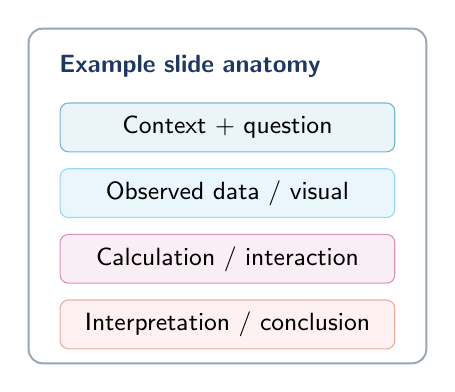
\begin{tikzpicture}[every node/.style={font=\small}]
  \node[
    draw=UTBlue!45,
    fill=white,
    rounded corners=5pt,
    line width=0.7pt,
    minimum width=5.05cm,
    minimum height=4.25cm,
    align=center,
    inner sep=8pt
  ] (box) {};
  \node[anchor=north west,text width=4.45cm,align=left] at ([xshift=0.28cm,yshift=-0.22cm]box.north west)
    {\textcolor{UTBlue}{\bfseries Example slide anatomy}};
  \node[draw=Pantone633!55,fill=Pantone633!8,rounded corners=3pt,minimum width=4.25cm,minimum height=0.62cm,anchor=north,align=center] (q) at ([yshift=-0.95cm]box.north) {Context + question};
  \node[draw=Pantone2985!70,fill=Pantone2985!15,rounded corners=3pt,minimum width=4.25cm,minimum height=0.62cm,below=0.20cm of q,align=center] (obs) {Observed data / visual};
  \node[draw=Pantone227!45,fill=Pantone227!7,rounded corners=3pt,minimum width=4.25cm,minimum height=0.62cm,below=0.20cm of obs,align=center] (calc) {Calculation / interaction};
  \node[draw=PantoneWarmRed!45,fill=PantoneWarmRed!7,rounded corners=3pt,minimum width=4.25cm,minimum height=0.62cm,below=0.20cm of calc,align=center] (con) {Interpretation / conclusion};
\end{tikzpicture}
\end{columns}
\end{frame}

% Slide 9
\begin{frame}{In-browser interactivity}
\vspace{0.25em}
\centering
\card{Pantone633}{Run R}{WebR lets students execute selected R code without leaving the slide deck or installing software locally.}
\hspace{0.25em}
\card{Pantone227}{Reveal thinking}{Fragment order controls when setup, calculation, and result appear during instruction.}
\hspace{0.25em}
\card{PantoneWarmRed}{Immediate checks}{Embedded quizzes and solution reveals provide quick formative feedback.}

\vspace{0.45em}
\begin{beamercolorbox}[rounded=true,sep=0.65em,wd=0.91\textwidth]{block body}
\centering
\textbf{Interaction principle:} each click should move the statistical reasoning forward.
\end{beamercolorbox}
\end{frame}

% Slide 10
\begin{frame}{A representative chapter structure}
\vspace{0.4em}
\begin{columns}[T,onlytextwidth]
\column{0.56\textwidth}
\begin{enumerate}
  \item Chapter opening and roadmap
  \item Core concept and notation
  \item Intuition before formal calculation
  \item Two applied examples
  \item Visual / graphical interpretation
  \item Check in R
  \item Short quiz or reflection
  \item Chapter summary and next-step navigation
\end{enumerate}

\column{0.40\textwidth}
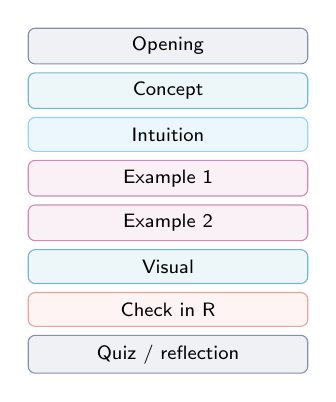
\begin{tikzpicture}[node distance=0.10cm]
  \node[draw=UTBlue!55,fill=UTBlue!7,rounded corners=2.5pt,minimum width=3.55cm,minimum height=0.43cm,align=center] (n1) {\scriptsize Opening};
  \node[draw=Pantone633!55,fill=Pantone633!7,rounded corners=2.5pt,minimum width=3.55cm,minimum height=0.43cm,align=center,below=of n1] (n2) {\scriptsize Concept};
  \node[draw=Pantone2985!75,fill=Pantone2985!14,rounded corners=2.5pt,minimum width=3.55cm,minimum height=0.43cm,align=center,below=of n2] (n3) {\scriptsize Intuition};
  \node[draw=Pantone227!50,fill=Pantone227!6,rounded corners=2.5pt,minimum width=3.55cm,minimum height=0.43cm,align=center,below=of n3] (n4) {\scriptsize Example 1};
  \node[draw=Pantone227!50,fill=Pantone227!6,rounded corners=2.5pt,minimum width=3.55cm,minimum height=0.43cm,align=center,below=of n4] (n5) {\scriptsize Example 2};
  \node[draw=Pantone633!55,fill=Pantone633!7,rounded corners=2.5pt,minimum width=3.55cm,minimum height=0.43cm,align=center,below=of n5] (n6) {\scriptsize Visual};
  \node[draw=PantoneWarmRed!50,fill=PantoneWarmRed!6,rounded corners=2.5pt,minimum width=3.55cm,minimum height=0.43cm,align=center,below=of n6] (n7) {\scriptsize Check in R};
  \node[draw=UTBlue!55,fill=UTBlue!7,rounded corners=2.5pt,minimum width=3.55cm,minimum height=0.43cm,align=center,below=of n7] (n8) {\scriptsize Quiz / reflection};
\end{tikzpicture}
\end{columns}
\end{frame}

% ============================================================
\section{From concept to classroom interaction}
% ============================================================

% Slide 11
\begin{frame}{Example 1: CONCEPT to visualization}
\screenshotplaceholder{Insert one of the strongest \textbf{concept + plot} slides.\\Suggested candidates: a confidence-interval visualization, power visualization, or regression example.}
\vspace{-0.25em}
\begin{itemize}
  \item Use this slide to show how the resource moves from \key{context} to \key{visual reasoning} before or alongside computation.
\end{itemize}
\end{frame}

% Slide 12
\begin{frame}{Example 2: Check in R}
\screenshotplaceholder{Insert a \textbf{Check in R / WebR} slide showing live browser-based computation and the solution interaction.}
\vspace{-0.25em}
\begin{itemize}
  \item Emphasize the connection between the hand-worked statistical method and its implementation in R.
  \item Check in R is especially valuable because STA258 tutorials require R, and this support also carries forward into upper-year statistics courses.
\end{itemize}
\end{frame}

% Slide 13
\begin{frame}{Example 3: formative feedback}
\screenshotplaceholder{Insert a \textbf{quiz or solution-reveal} slide that is visually clear and requires interpretation rather than rote calculation.}
\vspace{-0.25em}
\begin{itemize}
  \item The goal is not simply to reveal an answer, but to make the reasoning and common misconception visible.
\end{itemize}
\end{frame}

% Slide 14
\begin{frame}{Example 4: interactive statistical visualization}
\screenshotplaceholder{Insert a strong \textbf{Plotly / interactive visualization} slide.\\Suggested candidates: sampling distribution, hypothesis-test region, ANOVA/F distribution, or regression diagnostic.}
\vspace{-0.25em}
\begin{itemize}
  \item Use the interaction to reinforce what changes, what stays fixed, and what the graphical objects represent statistically.
\end{itemize}
\end{frame}

% ============================================================
\section{Development and refinement}
% ============================================================

% Slide 15
\begin{frame}{An iterative summer development process}
\vspace{0.6em}
\begin{center}
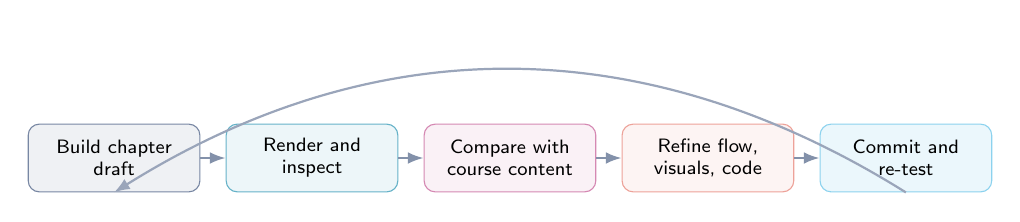
\begin{tikzpicture}[node distance=0.25cm and 0.32cm, every node/.style={font=\scriptsize}]
  \node[draw=UTBlue!60,fill=UTBlue!7,rounded corners=4pt,minimum width=2.18cm,minimum height=0.86cm,align=center] (a) {Build chapter\\draft};
  \node[draw=Pantone633!60,fill=Pantone633!7,rounded corners=4pt,minimum width=2.18cm,minimum height=0.86cm,align=center,right=of a] (b) {Render and\\inspect};
  \node[draw=Pantone227!50,fill=Pantone227!6,rounded corners=4pt,minimum width=2.18cm,minimum height=0.86cm,align=center,right=of b] (c) {Compare with\\course content};
  \node[draw=PantoneWarmRed!50,fill=PantoneWarmRed!6,rounded corners=4pt,minimum width=2.18cm,minimum height=0.86cm,align=center,right=of c] (d) {Refine flow,\\visuals, code};
  \node[draw=Pantone2985!80,fill=Pantone2985!14,rounded corners=4pt,minimum width=2.18cm,minimum height=0.86cm,align=center,right=of d] (e) {Commit and\\re-test};
  \foreach \x/\y in {a/b,b/c,c/d,d/e}{\draw[-{Latex[length=2mm]},thick,UTBlue!55] (\x)--(\y);}
  \draw[-{Latex[length=2mm]},thick,UTBlue!45,bend right=32] (e.south) to (a.south);
\end{tikzpicture}
\end{center}

\vspace{0.55em}
\begin{itemize}
  \item Refinement focused on \key{genuine instructional discrepancies}: incorrect formulas, broken interaction order, misleading wording, inconsistent examples, and serious layout issues.
  \item The workflow also standardized chapters without changing content simply for cosmetic uniformity.
\end{itemize}
\end{frame}

% Slide 16
\begin{frame}{What consistency work looked like}
\vspace{0.55em}
\begin{columns}[T,onlytextwidth]
\column{0.48\textwidth}
\textbf{Instructional consistency}
\begin{itemize}
  \item Example flow and fragment order
  \item Notation and final-answer precision
  \item R checks that match the worked example
  \item Conclusions stated in context
  \item Chapter-to-chapter navigation
\end{itemize}

\column{0.48\textwidth}
\textbf{Visual / technical consistency}
\begin{itemize}
  \item Fixed scaling and overflow
  \item Consistent Plotly presentation
  \item Readable axes and labels
  \item Solution / reset behavior
  \item Shared CSS and reusable layouts
\end{itemize}
\end{columns}

\vspace{0.75em}
\begin{beamercolorbox}[rounded=true,sep=0.85em,wd=\textwidth]{block body}
\centering
Consistency became a \textbf{course-level design problem}, not just a collection of isolated slide edits.
\end{beamercolorbox}
\end{frame}

% Slide 17
\begin{frame}{Designed for maintainability}
\vspace{0.6em}
\begin{columns}[T,onlytextwidth]
\column{0.54\textwidth}
\begin{itemize}
  \item Shared styling is centralized rather than duplicated across slides.
  \item Chapter files follow a predictable structure.
  \item A help manual documents rendering, navigation, WebR, quiz behavior, Git workflow, and common errors.
  \item The repository structure separates editable source from rendered output.
\end{itemize}

\column{0.42\textwidth}
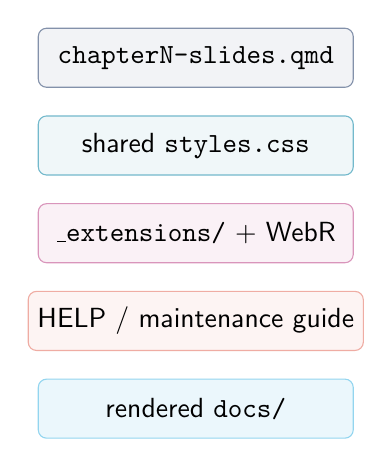
\begin{tikzpicture}[node distance=0.35cm]
  \node[draw=UTBlue!55,fill=UTBlue!6,rounded corners=3pt,minimum width=4.0cm,minimum height=0.75cm,align=center] (s1) {\texttt{chapterN-slides.qmd}};
  \node[draw=Pantone633!55,fill=Pantone633!6,rounded corners=3pt,minimum width=4.0cm,minimum height=0.75cm,align=center,below=of s1] (s2) {shared \texttt{styles.css}};
  \node[draw=Pantone227!45,fill=Pantone227!6,rounded corners=3pt,minimum width=4.0cm,minimum height=0.75cm,align=center,below=of s2] (s3) {\texttt{\_extensions/} + WebR};
  \node[draw=PantoneWarmRed!45,fill=PantoneWarmRed!6,rounded corners=3pt,minimum width=4.0cm,minimum height=0.75cm,align=center,below=of s3] (s4) {HELP / maintenance guide};
  \node[draw=Pantone2985!75,fill=Pantone2985!14,rounded corners=3pt,minimum width=4.0cm,minimum height=0.75cm,align=center,below=of s4] (s5) {rendered \texttt{docs/}};
\end{tikzpicture}
\end{columns}
\end{frame}

% Slide 18
\begin{frame}{What the project enables}
\vspace{0.25em}
\centering
\card{UTBlue}{For students}{A single browser-based path connecting explanation, visualization, computation, and formative practice.}
\hspace{0.25em}
\card{Pantone633}{For instructors}{Reusable teaching sequences with controlled reveal order, consistent examples, and integrated R demonstrations.}
\hspace{0.25em}
\card{Pantone227}{For future developers}{A documented structure that can be updated chapter-by-chapter without rebuilding the entire system.}

\vspace{0.45em}
\begin{beamercolorbox}[rounded=true,sep=0.6em,wd=0.9\textwidth]{block body}
\centering
The contribution is both \textbf{instructional} and \textbf{infrastructural}: the content and the system used to deliver it are developed together.
\end{beamercolorbox}
\end{frame}

% ============================================================
\section{Limitations and future work}
% ============================================================

% Slide 19
\begin{frame}{Limitations}
\vspace{0.7em}
\begin{itemize}
  \item The resource is still in development and has not yet been fully evaluated through live course deployment.
  \item Browser-based interactivity introduces dependencies on rendering, JavaScript, and WebR behavior across devices.
  \item Interactive slides require more maintenance than static lecture material because code, styling, and pedagogy must remain synchronized.
  \item Accessibility and mobile responsiveness require continued testing as the resource evolves.
\end{itemize}
\end{frame}

% Slide 20
\begin{frame}{Future work}
\vspace{0.6em}
\begin{center}
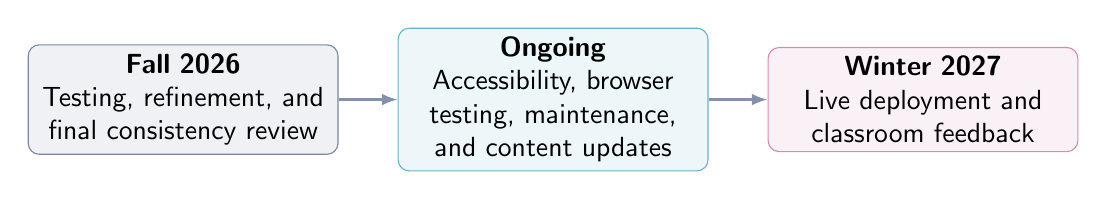
\begin{tikzpicture}[node distance=0.45cm and 0.75cm]
  \node[draw=UTBlue!60,fill=UTBlue!7,rounded corners=4pt,text width=3.7cm,minimum height=1.25cm,align=center] (f1) {\textbf{Fall 2026}\\Testing, refinement, and final consistency review};
  \node[draw=Pantone633!60,fill=Pantone633!7,rounded corners=4pt,text width=3.7cm,minimum height=1.25cm,align=center,right=of f1] (f2) {\textbf{Ongoing}\\Accessibility, browser testing, maintenance, and content updates};
  \node[draw=Pantone227!50,fill=Pantone227!6,rounded corners=4pt,text width=3.7cm,minimum height=1.25cm,align=center,right=of f2] (f3) {\textbf{Winter 2027}\\Live deployment and classroom feedback};
  \draw[-{Latex[length=2mm]},thick,UTBlue!55] (f1)--(f2);
  \draw[-{Latex[length=2mm]},thick,UTBlue!55] (f2)--(f3);
\end{tikzpicture}
\end{center}

\vspace{1.0em}
\begin{itemize}
  \item Use classroom feedback to determine which interactions genuinely support learning and which should be simplified.
  \item Continue developing the resource as a maintainable course platform rather than a one-time slide deck.
\end{itemize}
\end{frame}

% Slide 21
\begin{frame}{Takeaways}
\vspace{0.75em}
\begin{enumerate}
  \item \textbf{Quarto provides a single authoring environment} for text, mathematics, R, HTML/CSS, and interactive presentation components.
  \item \textbf{Interactivity is most useful when it follows the statistical reasoning}, rather than being added as a separate feature.
  \item \textbf{Consistency across chapters matters pedagogically}: students can focus on the concept when the structure and interaction patterns are predictable.
  \item \textbf{Maintainability is part of instructional design}: future course updates should be possible without reconstructing the system.
\end{enumerate}
\end{frame}

% Slide 22
\section{Acknowledgements}
\begin{frame}{Acknowledgements}
\vspace{0.7em}
We would like to thank:
\begin{itemize}
  \item the Department of Mathematical and Computational Sciences at the University of Toronto Mississauga;
  \item everyone who provided feedback during the development and refinement of the STA258 resources;
  \item additional acknowledgements to be finalized for the presentation.
\end{itemize}
\end{frame}

% Slide 23
\begin{frame}[allowframebreaks]{References}
\scriptsize
\begin{thebibliography}{99}

\bibitem{sta258resource}
Mudalige, N., Selvapandian, A., \& Halime, S. (2026).
\newblock \textit{STA258: Statistics with Applied Probability -- Interactive instructional resources}.
\newblock University of Toronto Mississauga. [Quarto course resource / e-book; final URL to be added.]

\bibitem{alili2025}
Alili, N., \& Su, X. (2025).
\newblock Student-faculty co-creation of open educational resources for learning applied statistics with open source software tools.
\newblock \textit{Journal of Computing, Data, and Exploration, 1}(1).
\newblock \url{https://doi.org/10.33137/codex.v1i1.45881}

\bibitem{asa2016}
American Statistical Association Revision Committee. (2016).
\newblock \textit{Guidelines for Assessment and Instruction in Statistics Education (GAISE) College Report 2016}.
\newblock American Statistical Association.
\newblock \url{https://www.amstat.org/asa/files/pdfs/gaise/gaisecollege_full.pdf}

\bibitem{quarto}
Posit. (n.d.).
\newblock \textit{Quarto documentation}.
\newblock \url{https://quarto.org/docs/}

\bibitem{webr}
R-universe / WebR Project. (n.d.).
\newblock \textit{WebR: R in the browser}.
\newblock \url{https://docs.r-wasm.org/webr/latest/}

\bibitem{rfoundation}
R Foundation. (n.d.).
\newblock \textit{R: The R Project for Statistical Computing}.
\newblock \url{https://www.r-project.org/}

\bibitem{utmsta258}
University of Toronto Mississauga. (n.d.).
\newblock \textit{STA258H5: Statistics with Applied Probability}.
\newblock Academic Calendar.
\newblock \url{https://utm.calendar.utoronto.ca/course/sta258h5}

\end{thebibliography}
\end{frame}

% Slide 24 -- End
\begin{frame}[plain]
\begin{tikzpicture}[remember picture,overlay]
  \fill[SoftGrey] (current page.south west) rectangle (current page.north east);
  \fill[UTBlue] (current page.north west) rectangle ([yshift=-0.16cm]current page.north east);
  \fill[Pantone633] (current page.south west) rectangle ([yshift=0.12cm]current page.south east);
\end{tikzpicture}

\vspace*{0.35em}

\includegraphics[width=0.21\paperwidth]{UTM-MCS-logo-transparent.png}

\vfill
\begin{center}
{\ttfamily\fontsize{28}{32}\selectfont\color{UTBlue}\textbf{Thank you.}}\\[1.1em]
{\large\color{Pantone633}Questions or comments?}
\end{center}
\vfill
\begin{flushright}

\includegraphics[width=0.13\paperwidth]{STA258_cat_logo.png}\hspace*{0.6em}
\end{flushright}
\vspace{0.25em}
\end{frame}

\end{document}
